\section{Concepts of a Reinforcement Learning System} \label{sec:rlconcepts}

Reinforcement Learning is learning what to do -- how to map situations to actions -- so as to maximize
a numerical reward signal. The learner is not told which actions to take, but instead must discover
which actions yield the most reward by trying them. In the most interesting and challenging cases,
actions may affect not only the immediate reward but also the next situation and, through that, all
subsequent rewards \cite{sutton1998rli}.

This learning process happens by interacting with the environment where the agent lives and therefore choose its actions. It is basically a "trial and error" approach as humans or other animals do, but in this case using a computational approach and mathematical modeling.

The origin of modern Reinforcement Learning has two main threads developed outside Artificial Intelligence research. One concerns about trial and error search inside psychology of animal learning, based on Behaviorism theory \cite{skinner1953science} and "The Law of Effect" \cite{Thorndike173}. The other thread concerns the problem of optimal control and its solution using value functions
and dynamic programming. Both of them contributed for the modern ideas in reinforcement learning, either with the abstractions of learning or mathematical modeling for this problem.

Reinforcement Learning is different from other kinds of Machine Learning, for several reasons:

\begin{itemize}
	\item \textbf{There is no supervisor, only a reward signal}: In Supervised Learning, there is a set of pairs $(x, y)$ and we optimize a cost function in a way to minimize the error from prediction and the ground truth. Therefore, there is a knowledgable external supervisor and a clear specification of mapping between situation and action to take - which doesn't exist in the context of reinforcement.
	
	\item \textbf{Feeback is delayed, not instantaneous}: In Reinforcement Learning, the reward is a consequence of a sequence of actions, rather than a direct mapping from actions to reward. For example, during the learning of a kick motion, the final reward of ball movement only occurs after all the agent motion control.
	
	\item \textbf{Data is not independent and identically distributed}: In this kind of learning, there is a intrinsic sequentiality, i.e, the data we collect at some point depends on the state we are.
	
	\item \textbf{Agent's actions affect the subsequent data it receives}: More than being i.i.d data, the learning process itself change the data distribution, differently from supervised learning where the dataset doesn't change during the course of training.
\end{itemize}


Therefore, the optimization problem in Reinforcement Learning has new challenges and needs a different analysis when compared with other kinds of Machine Learning. In this chapter, we will explore these ideas and state-of-art techniques to sustain our experimentations.

\section{Reinforcement Learning System}\label{sec:rlsystem}

Figure \ref{fig:rlsystem} shows how a Reinforcement Learning system works and some of the core concepts involved. As described in section \ref{sec:rlconcepts}, there are two main entities in Reinforcement Learning: an \textit{agent}, which takes actions with the object of accumulate reward, and a \textit{environment}, the place where happens this interaction and whose dynamics affects the decision about these actions.

During learning process, the agents gets a \textit{observation} from the environment and maps to a \textit{state}. Accordingly to that state, the agent then executes an \textit{action} in the environment, based on the current \textit{policy} of actions, which has a consequence in the environment and causes a transition in that state. Furthermore, the agent receives a \textit{reward} signal about how that action affected the environment in terms of accomplish the task goals. This cycle will happen iteratively and the policy will be adjusted until in a way that maximize the cumulative reward.

In the next subsections, we will describe in deep the main concepts of a RL system.

\begin{figure}[!htpb]
	\centering
	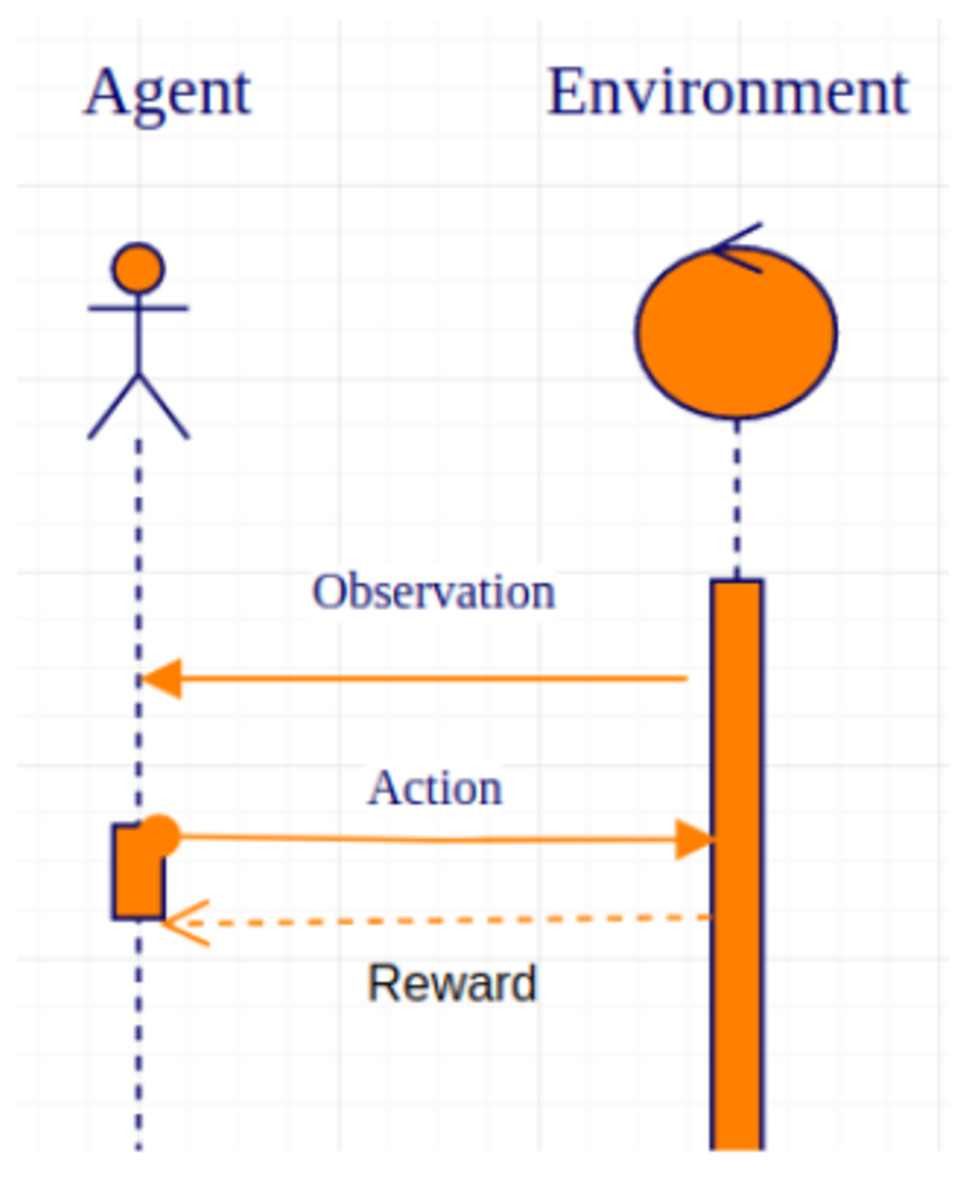
\includegraphics[scale=0.5]{Cap4/rlsystem.eps}
	\caption{Reinforcement Learning System.}
	\label{fig:rlsystem}
\end{figure}

\subsection{Reward}\label{sec:reward}
A reward signal is a scalar number received by the agent and drives the goal in a RL problem. It indicates how well the action taken is in that state. In the learning process, the reward signal guides the policy modification: when an actions has high reward, it is a case of positive reinforcement and the policy will be adjusted to take this action more likely in that state; on the other side, if the reward is low, it is a case of negative reinforcement and policy will try to act in this way less times.

Finally, we can formalize this idea stating that RL is based on the \textbf{Reward Hypothesis}:

\begin{definition}
	All goals can be described by the maximization of expected cumulative reward.
\end{definition}

\subsection{State}

Basically, a state is a function of the sequence observations, actions and rewards. There are two different concepts of State:

\begin{itemize}
	\item \textbf{Environment State}: Environment's internal representation - the way it understands its feature at that point and uses to pick next observation or reward.
	\item \textbf{Agent State}: The information that agent perceives and understand from the observation and uses to pick a new action.
\end{itemize}

In RL problems, we commonly use the \textbf{Agent State} concept -- the information provided by the environment and interpreted by the agent in order to decide which action to take next. More specifically, we will use the concept of Markov state, which will be discussed later.

\subsection{Policy}

A policy defines the agent's behavior. It maps state to actions. It corresponds to what in psychology would be called a set of stimulus–response rules or associations \cite{sutton1998rli}. 

The policy is the core element of a RL system. It is sufficient to define the behavior of an agent and therefore is the piece we need after the learning process. There are two kind of policies:

\begin{itemize}
	\item \textbf{Deterministic Policy}, where there is a direct map from state to action:
	
	\begin{equation}
	a = \pi(s)
	\end{equation}
	
	\item \textbf{Stochastic Policy}, where the map happens from the static to a probability distribution between actions:
	
	\begin{equation}
	\pi (a | s) = \mathbb{P}[A_{t} = a | S_{t} = s]
	\end{equation}
\end{itemize}

\subsection{Value Function}
Whereas the reward signal indicates what is good in an immediate sense, a value function specifies what is good in the long run. The value function is a estimate of reward the agent can expect to accumulate over the future, until a terminal state. 

The value function can be formalized in Equation \ref{eq:valuefunction}:

\begin{equation}\label{eq:valuefunction}
v_{\pi}(s) = \mathbb{E}_{\pi}[R_{t+1} + \gamma R_{t+2} + \gamma^{2} R_{t + 3} + ... | S_{t} = s]
\end{equation}

In RL, we focus on choosing actions that bring about states of highest value, not just highest reward. Therefore, it is common to sacrifice immediate rewards to maximize future rewards.

Furthermore, it is much harder to determine value than rewards, because while this is given directly from the environment, that one must be estimated accordingly to data the agent receives. We will describe state-of-art algorithms to predict value function later.

\subsection{Model}

A model is a component that predicts environment's behavior. Basically it will estimate the next state given the agent's action, as formalized in Equation \ref{eq:modelrl}:

\begin{equation}\label{eq:modelrl}
\mathcal{P}_{ss'}^{a} = \mathbb{P}[S_{t+1} = s' | S_{t} = s, A_{t} = a]
\end{equation}

Where $\mathcal{P}$ is a transition matrix which calculates the probability of transit between state $s$ and $s'$ given the action $a$.

Models are used for planning, by which we
mean any way of deciding on a course of action by considering possible future situations before they are
actually experienced \cite{sutton1998rli}.

There are two methods based on model classification:

\begin{itemize}
	\item \textbf{Model-based RL}, methods that uses model and planning to solve the learning challenge;
	\item \textbf{Model-free RL}, which are methods that are direct trial and error learners.
\end{itemize}

Sometimes there is no model of the environment or it is very hard to create it -- in that cases, we commonly use model-free methods. In this work, we don't know about the dynamics of simulator, thus we adopt model-free RL.

\section{Markov Decision Process}

 Markov Decision Processes (MDPs) are a classical
formalization of sequential decision making, where actions influence not just immediate rewards, but also
subsequent situations, or states, and through those future rewards \cite{sutton1998rli}. Thus, MDPs formally describe an environment for Reinforcement Learning. Almost all RL problems can be formalized as MDPs \cite{davidsilverlec2}.

In next subsections, we will define mathematically what is a MDP, its major components and properties.

\subsection{Markov State}\label{sec:markovstate}

A state $S_{t}$ is considered \textit{Markov State} if and only if:

\begin{equation}\label{eq:markovstate}
	\mathbb{P}[S_{t+1} | S_{t}] = \mathbb{P}[S_{t+1} | S_{1},\dots, S_{t}]
\end{equation}

Intuitively, Equation \ref{eq:markovstate} tells that in a Markov State, the future is independent of the past given the present. It means that the state has all the relevant information from the history and therefore it is sufficient statistic for the future. 

As example, consider a chess game: given a specific state -- a set of pieces in the board -- all the information a player needs to play is in the board state, regardless of how the game came in that circumstance. The history may be thrown away.

\subsection{State Transition Matrix}\label{sec:statetransition}

Other major component of a MDP is the State Transition Matrix. Given a set of Markov States, this component defines the probabilities of transition between states. More formally:

\begin{equation}
\mathcal{P} = \begin{bmatrix}
\mathcal{P}_{11} &  \dots  & \mathcal{P}_{1n} \\
\vdots \\
\mathcal{P}_{n1} &  \dots  & \mathcal{P}_{nn} 
\end{bmatrix}
\end{equation}

Where $\mathcal{P}_{ss'}$ is the transition probability:

\begin{equation}
\mathcal{P}_{ss'} = \mathbb{P}[S_{t+1} = s' | S_{t} = s]
\end{equation}

\subsection{Markov Decision Process}

Using the concepts from subsecions \ref{sec:markovstate} and \ref{sec:statetransition}, we can define a \textit{Markov Process} (MP):

\begin{definition}
	A Markov Process, or Markov Chain, is a tuple $(\mathcal{S}, \mathcal{P})$, where:
	\begin{itemize}
		\item $\mathcal{S}$ is a set of states; and
		\item $\mathcal{P}$ is the state transition probability matrix.
	\end{itemize}
\end{definition}

Considering the definition of Markov Process and the concept of Reward described in section \ref{sec:reward}, we can define a \textit{Markov Reward Process} (MRP):

\begin{definition}
	A Markov Reward Process, is a tuple $(\mathcal{S}, \mathcal{P}, \mathcal{R}, \gamma)$, where:
	\begin{itemize}
		\item $\mathcal{S}$ is a set of states; 
		\item $\mathcal{P}$ is the state transition probability matrix;
		\item $\mathcal{R}$ is a reward function, i.e, $\mathcal{R}_{s} = \mathbb{E}[R_{t+1} | S_{t} = s]$; and
		\item $\gamma$ is a discount factor, where $\gamma \in [0,1]$
	\end{itemize}
\end{definition}

A Markov Reward Process (MRP) describes mathematically an environment in a RL problem. Furthermore, we can differentiate an MRP from a MP by the concept of \textit{Return} that is directly related to the reward over time:

\begin{equation}
G_{t} = R_{t+1} + \gamma R_{t + 2} + \dots = \sum_{k = 0}^{\infty} \gamma^{k} R_{t + k + 1}
\end{equation}

The idea around cumulative reward was described earlier in section \ref{sec:rlsystem}. However, we need to analyze the discount factor $\gamma$ -- it will weight the trade-off between immediate and delayed rewards. 

Basically, if $\gamma$ is close to zero, the MRP will consider more an immediate reward; on the other side, if $\gamma$ is close to one, the MRP will consider more a delayed reward. Furthermore, the idea of discount is mathematically convenient and avoids infinite returns in cyclic Markov processes \cite{davidsilverlec2}.

Finally, we can extend the idea of MRP by adding an decision making procedure execute by the agent -- which results in the concept of \textit{Markov Decision Process}:

\begin{definition}
		A Markov Decision Process, is a tuple $(\mathcal{S}, \mathcal{A}, \mathcal{P}, \mathcal{R}, \gamma)$, where:
	\begin{itemize}
		\item $\mathcal{S}$ is a set of states; 
		\item $\mathcal{A}$ is a set of actions; 
		\item $\mathcal{P}$ is the state transition probability matrix;
		\item $\mathcal{R}$ is a reward function, i.e, $\mathcal{R}_{s} = \mathbb{E}[R_{t+1} | S_{t} = s]$; and
		\item $\gamma$ is a discount factor, where $\gamma \in [0,1]$
	\end{itemize}
\end{definition}

Thus, MDP is a MRP with decisions. It worth to mention that the state transition probability $\mathcal{P}$ in MDP also takes in consideration the action executed by the agent:

\begin{equation}
\mathcal{P}_{ss'}^{a} = \mathbb{P}[S_{t+1} = s' | S_{t} = s, A_{t} = a]
\end{equation}

Now, we have a formal definition of a RL problem by using MDP concept. Figure \ref{fig:mdprlsystem} shows the agent-environment interaction in a MDP. In the next section, we will formalize other RL components such as Value Function and Policy in a MDP context.

\begin{figure}[ht!]
	\centering
	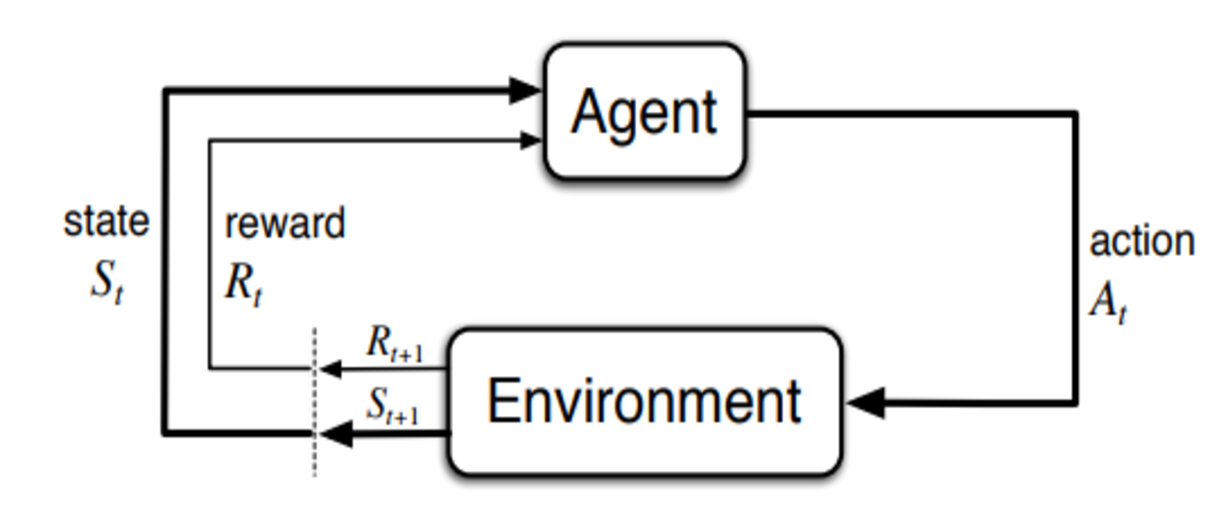
\includegraphics[scale=0.5]{Cap4/mdprlsystem.eps}
	\caption{The agent–environment interaction in a Markov decision process \cite{sutton1998rli}.}
	\label{fig:mdprlsystem}
\end{figure}

\subsection{Value Function and Policy}

